\setauthor{Benjamin Ecker}

In diesem Kapitel werden alle Funktionalität der App erklärt und wer darauf Zugriff hat. Das Kapitel ist so gegliedert, dass es beim durchlesen den gesamten Ablauf der Turniererstellung, wie Durchführung erklärt, aber auch immer als Nachschlaghilfe für einzelene Pages dient.

\section{Home-Page - Rollen:Alle}
\begin{figure}[H]
    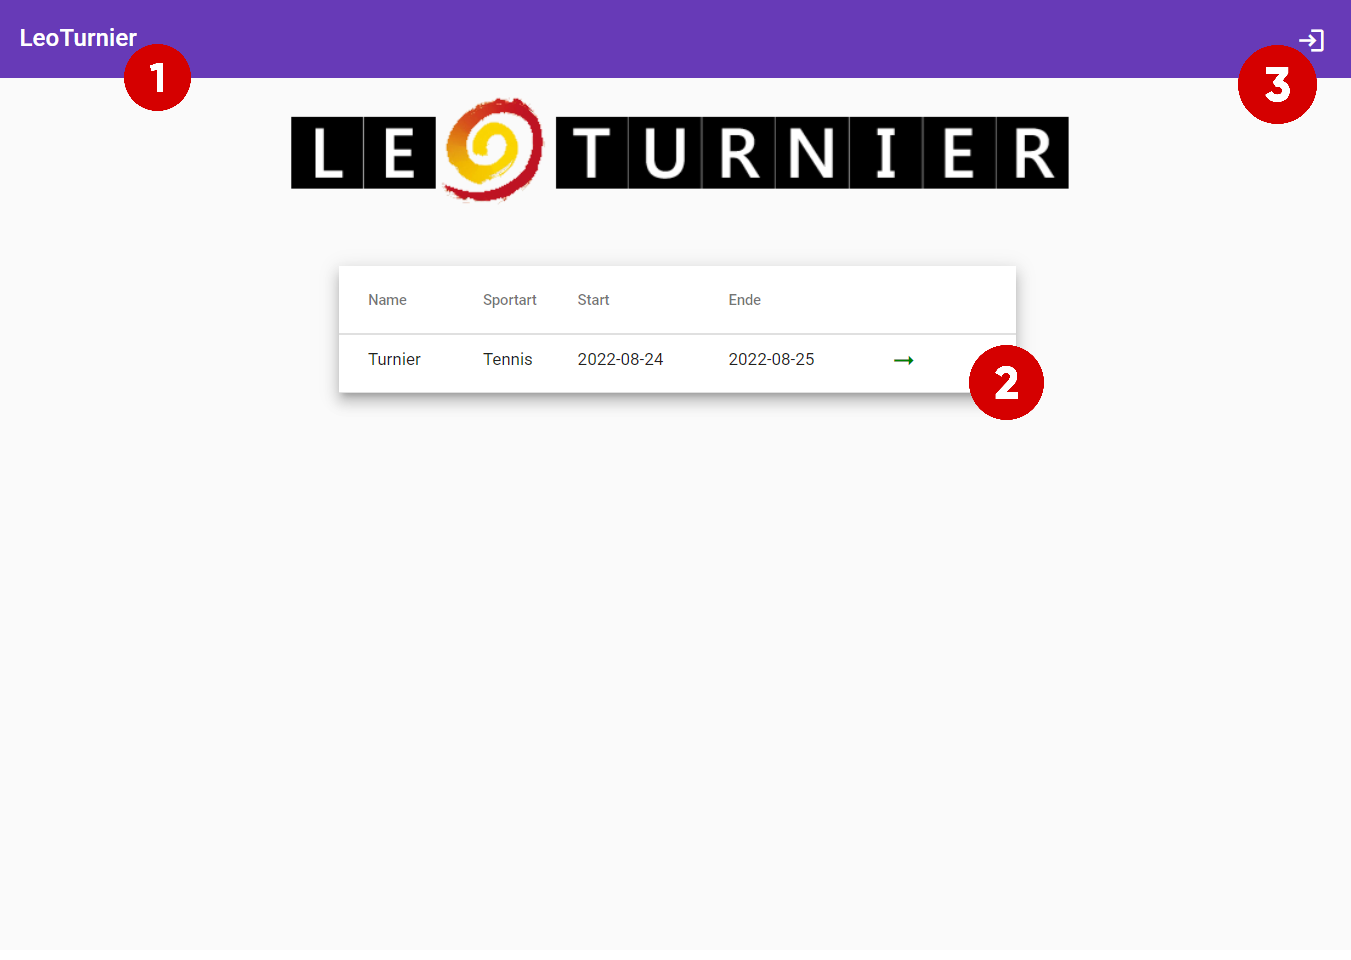
\includegraphics[scale=0.4]{pics/user-guide/homepage.png}
    \caption{Homepage}
\end{figure}
\bigskip


\includegraphics[scale=0.05]{pics/user-guide/numbers/number-1.png} \begin{LARGE} Titel \end{LARGE}

Links oben wird dauerhaft der Titel LeoTurnier gezeigt dieser dient auch gleichzeitig als Homebutton,
also kommt man per Knopfdruck immer wieder auf diese Seite.
\bigskip



\includegraphics[scale=0.05]{pics/user-guide/numbers/number-2.png} \begin{LARGE} Laufenden Turniere \end{LARGE}

In dieser Tabelle werden alle laufenden Turniere angezeigt. Zu jedem Turnier werden die Sportart, das Startdatum und das Enddatum angezeigt,
sollten diese eingetragen sein. (\textit{Nur der Name und der Modus sind zur Erstellung nötig})

Mit dem rechten grünen Pfeil kommen Sie zur Tournament-View-Page(5.2) des jeweiligen Turniers.
\bigskip

\newpage

\includegraphics[scale=0.05]{pics/user-guide/numbers/number-3.png} \begin{LARGE} Login Button \end{LARGE}

Um Turniere zu erstellen und verwalten zu können ist es nötig sich vorher einzuloggen. Mit diesem Button sollten Sie direkt zum Keycloak weitergeleitet werden um sich mit ihrem Username und Password zu authorisieren.
Danach werden Sie zur Login-Page(5.3) weitergeleitet werden.

\newpage
\section{Tournament-View-Page - Rollen: Alle}

Es gibt 2 Arten von Tournament-View-Pages:
\begin{itemize}
    \item Tree-View (für den Elimination Modus)
    \item Table-View (für den Round Robin Modus)
\end{itemize}

\subsection{Tree-View}
\begin{figure}[H]
    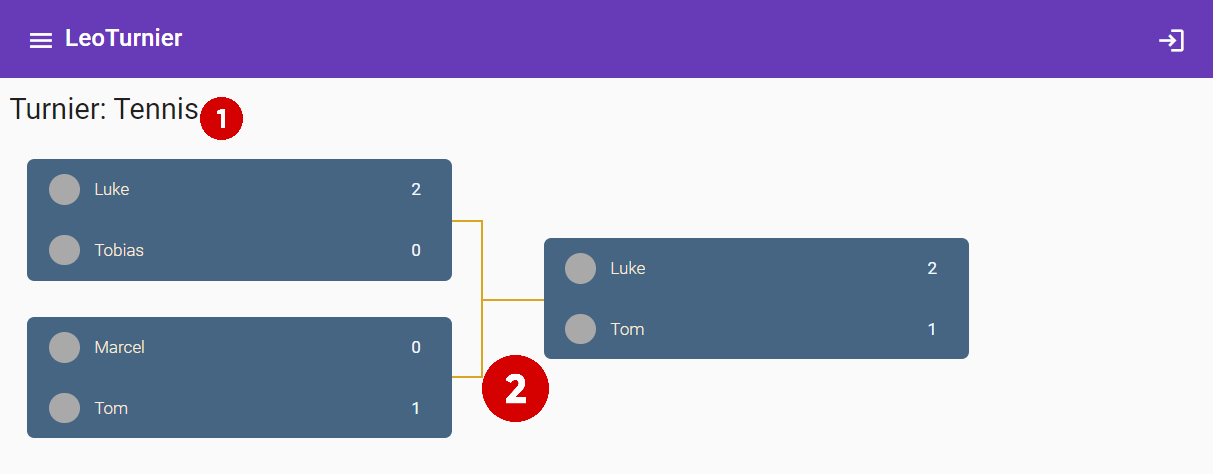
\includegraphics[scale=0.4]{pics/user-guide/tree-view.png}
    \caption{Tree-View}
\end{figure}
\bigskip


\includegraphics[scale=0.05]{pics/user-guide/numbers/number-1.png} \begin{LARGE} Info \end{LARGE}

Hier finden Sie eine kurze Info zum Turniernamen und Sportart
\bigskip


\includegraphics[scale=0.05]{pics/user-guide/numbers/number-2.png} \begin{LARGE} Turnierbaum \end{LARGE}

Hier finden Sie den Turnierbaum, dieser zeigt alle Ergebnisse bzw. aktuellen Spielstände eines Turnieres an.
Im Screenshot sehen Sie eine der einfachsten Formen eines Turnierbaums mit 4 Spielern. Sollte der Turnierbaum bei
steigender Spieleranzahl zu groß werden um alles auf einen Bildschirm zu sehen verwenden Sie bitte den Slider am unterem Bildschirmrand.

Das Neuladen des Turniers funktioniert auf dieser Seite nicht. Um den aktuellsten Stand des Turniers zu bekommen navigieren Sie zurück auf die Home-Page und wieder auf den grünen Pfeil.

\bigskip
\subsection{Table-View}
\begin{figure}[H]
    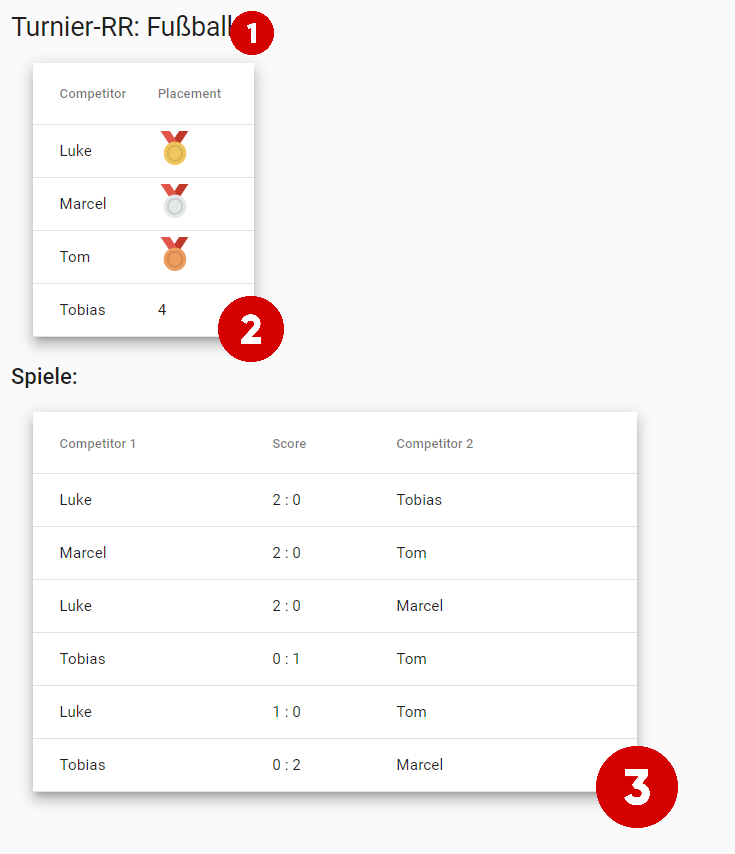
\includegraphics[scale=0.5]{pics/user-guide/table-view.PNG}
    \caption{Table-View}
\end{figure}
\bigskip

\includegraphics[scale=0.05]{pics/user-guide/numbers/number-1.png} \begin{LARGE} Info \end{LARGE}

Hier finden Sie eine kurze Info zum Turniernamen und Sportart

\bigskip

\includegraphics[scale=0.05]{pics/user-guide/numbers/number-2.png} \begin{LARGE} Platzierungen \end{LARGE}

In dieser Tabelle werden alle Spieler, nach Placement aufsteigend sortiert, angezeigt.

\bigskip

\includegraphics[scale=0.05]{pics/user-guide/numbers/number-3.png} \begin{LARGE} Spiele \end{LARGE}

In dieser Tabelle werden alle Ergebnisse bzw. aktuellen Spielstände eines Turnieres angezeigt.
Die ersten drei Plätze erhalten dabei auch eine Medaille.

\newpage
\section{Login-Page - Rollen: Admin,Tournament-Organizer}
\begin{figure}[H]
    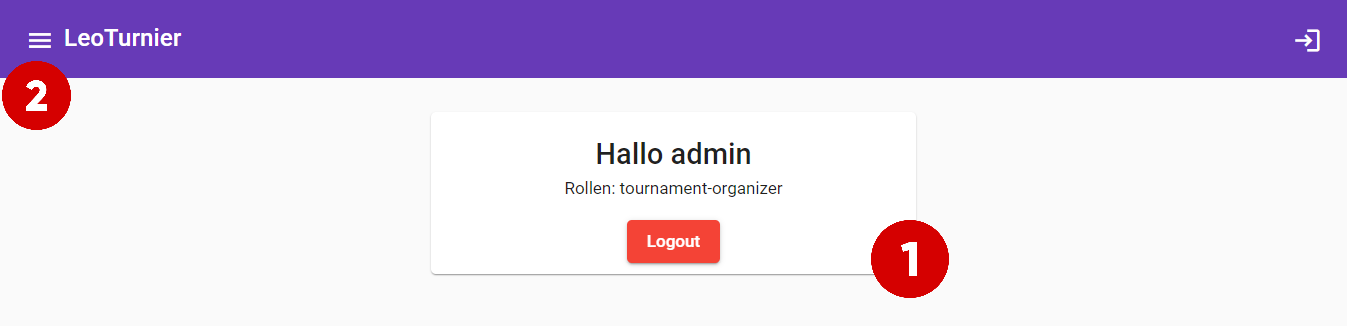
\includegraphics[scale=0.4]{pics/user-guide/login-page.PNG}
    \caption{Login-Page}
\end{figure}
\bigskip


\includegraphics[scale=0.05]{pics/user-guide/numbers/number-1.png} \begin{LARGE} Rollen und Logout Button \end{LARGE}

Hier finden Sie alle Ihnen zugewiesenen Rollen sowie einen Logout-Button der ihre Session beendet und Sie zurück zur Home-Page leitet.
\bigskip


\includegraphics[scale=0.05]{pics/user-guide/numbers/number-2.png} \begin{LARGE} Navigation-Burger \end{LARGE}

Nachdem Sie jetzt eingeloggt sind erscheint oben rechts ein Nav-Burger. Per Knopfdruck zeigt dieser Ihnen nun eine Liste aller Pages die zur
Turnierverwaltung nötig sind.

\newpage
\section{Player-Page - Rollen:Admin,Tournament-Organizer}
\begin{figure}[H]
    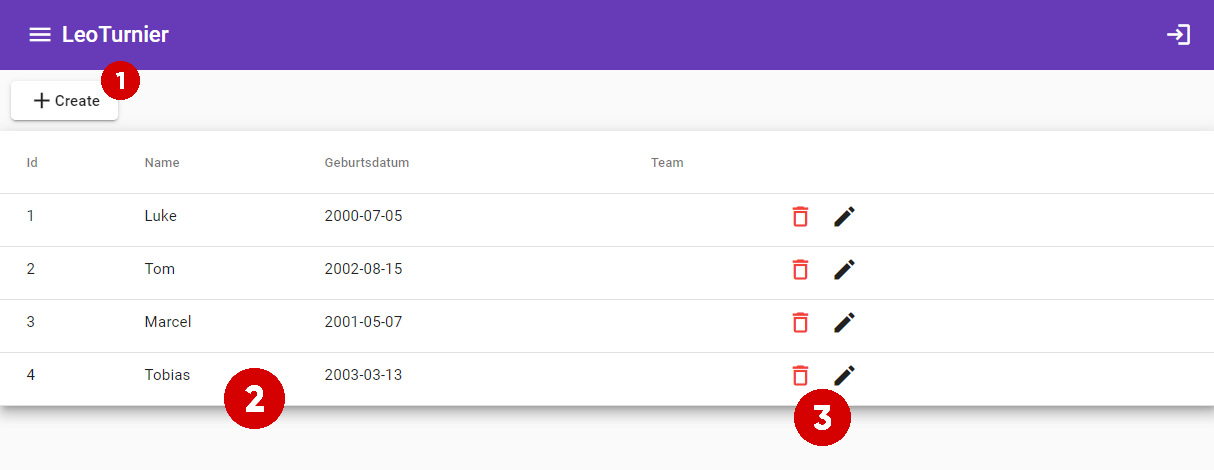
\includegraphics[scale=0.425]{pics/user-guide/player-overview-page.PNG}
    \caption{Player-Overview-Page}
\end{figure}
\bigskip


\includegraphics[scale=0.05]{pics/user-guide/numbers/number-1.png} \begin{LARGE} Create-Button \end{LARGE}

Button zum Erstellen neuer Spieler und leitet Sie zur Player-Details-Page(5.4.1).

\bigskip

\includegraphics[scale=0.05]{pics/user-guide/numbers/number-2.png} \begin{LARGE} Players \end{LARGE}

In dieser Tabelle werden alle Spieler mit ihren Details angezeigt. Zu jedem Spieler werden hier seine Id, Name, Geburtsdatum und zugehöriges Team angezeigt,
sollten dieser vorhanden sein. (\textit{Nur der Name ist zur Erstellung nötig})

\bigskip

\includegraphics[scale=0.05]{pics/user-guide/numbers/number-3.png} \begin{LARGE} Actions \end{LARGE}

Diese Spalte beinhaltet zwei Icon-Buttons:
\begin{itemize}
    \item 
\includegraphics[scale=0.3]{pics/user-guide/delete-icon.PNG} Löschen eines Spielers (Sie müssen diese Aktion zwei mal bestätigen)
    \item
\includegraphics[scale=0.3]{pics/user-guide/edit-icon.PNG}Updaten eines Spielers(Sie werden danach zur Player-Details-Page(5.4.1)geleitet)
\end{itemize}
\subsection{Player-Details-Page}
\begin{figure}[H]
    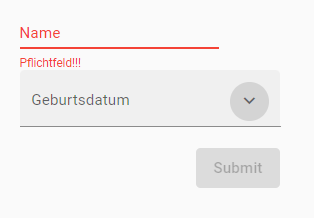
\includegraphics[scale=0.8]{pics/user-guide/player-create-page.PNG}
    \caption{Player-Details-Page}
\end{figure}

Diese Page ist zum Erstellen und Updaten von Spielern. Die Mindestanforderungen sind hierbei nur ein Name.


\section{Team-Page - Rollen:Admin,Tournament-Organizer}
\begin{figure}[H]
    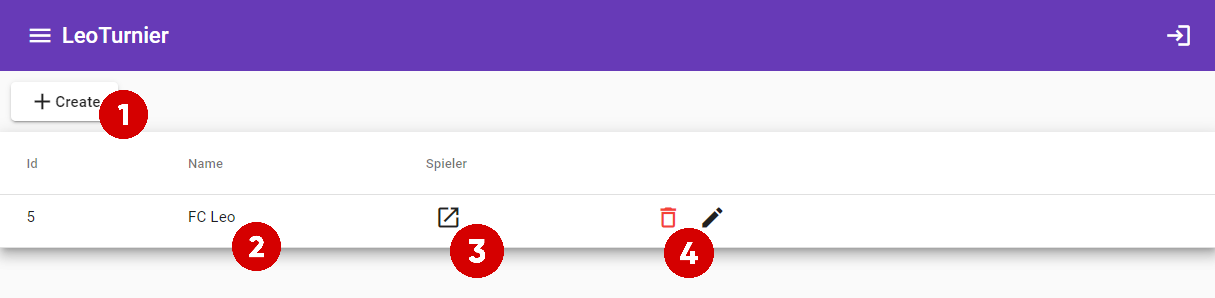
\includegraphics[scale=0.44]{pics/user-guide/team-overview-page.PNG}
    \caption{Team-Overview-Page}
\end{figure}
\bigskip


\includegraphics[scale=0.05]{pics/user-guide/numbers/number-1.png} \begin{LARGE} Create-Button \end{LARGE}

Button zum Erstellen neuer Teams und leitet Sie zur Team-Details-Page(5.5.1).

\bigskip

\includegraphics[scale=0.05]{pics/user-guide/numbers/number-2.png} \begin{LARGE} Teams \end{LARGE}

In dieser Tabelle werden alle Teams mit ihren Details angezeigt. Zu jedem Team werden hier seine Id, Name und zugehörige Spieler angezeigt,
sollten dieser vorhanden sein. (\textit{Nur der Name ist zur Erstellung nötig})

\bigskip

\includegraphics[scale=0.05]{pics/user-guide/numbers/number-3.png} \begin{LARGE} Spieler \end{LARGE}

In der Spalte Spieler finden Sie einen Icon-Button zu einem PopUp-Fenster welches eine Liste aller Spieler des Teams anzeigt.

\begin{figure}[H]
    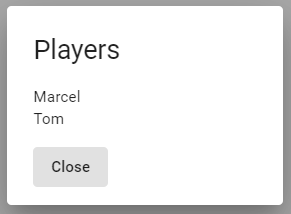
\includegraphics[scale=0.5]{pics/user-guide/teams-player-popup.PNG}
    \caption{Team-Players-PopUp}
\end{figure}

\bigskip

\includegraphics[scale=0.05]{pics/user-guide/numbers/number-4.png} \begin{LARGE} Actions \end{LARGE}

Diese Spalte beinhaltet zwei Icon-Buttons:
\begin{itemize}
    \item 
\includegraphics[scale=0.3]{pics/user-guide/delete-icon.PNG} Löschen eines Teams (Sie müssen diese Aktion zwei mal bestätigen)
    \item 
\includegraphics[scale=0.3]{pics/user-guide/edit-icon.PNG}Updaten eines Teams(Sie werden danach zur Team-Details-Page(5.5.1) geleitet)
\end{itemize}

\bigskip
\subsection{Team-Details-Page}
\begin{figure}[H]
    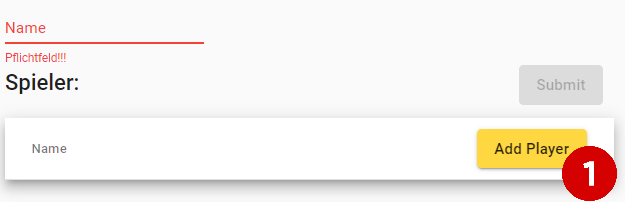
\includegraphics[scale=0.5]{pics/user-guide/team-create-page.PNG}
    \caption{Team-Details-Page}
\end{figure}
Diese Page ist zum Erstellen und Updaten von Spielern. Die Mindestanforderungen sind hierbei nur ein Name.

\bigskip

\includegraphics[scale=0.05]{pics/user-guide/numbers/number-1.png} \begin{LARGE} Add-Player \end{LARGE}

Bei Knopfdruck des Add-Player Button erscheint eine Liste aller Spieler die nicht in dem Team sind.
(\textit{Keine mehrfach Auswahl}) 

\begin{figure}[H]
    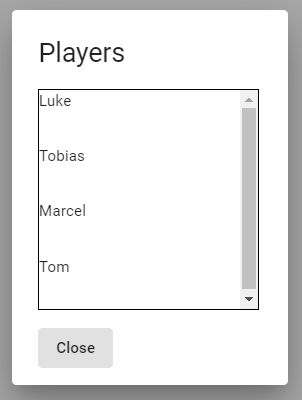
\includegraphics[scale=0.5]{pics/user-guide/add-player.PNG}
    \caption{Add-Player-PopUp (Team)}
\end{figure}

\newpage
\section{Tournament-Page Rollen:Admin,Tournament-Organizer}
\begin{figure}[H]
    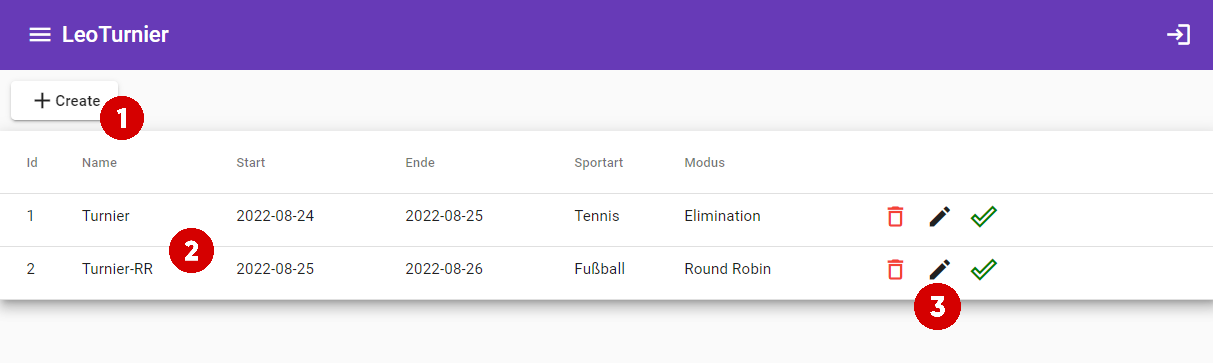
\includegraphics[scale=0.4]{pics/user-guide/tournament-overview-page.PNG}
    \caption{Tournament-Overview-Page}
\end{figure}


\includegraphics[scale=0.05]{pics/user-guide/numbers/number-1.png} \begin{LARGE} Create-Button \end{LARGE}

Button zum Erstellen neuer Tournaments und leitet Sie zur Tournament-Details-Page(5.6.1).

\bigskip

\includegraphics[scale=0.05]{pics/user-guide/numbers/number-2.png} \begin{LARGE} Tournaments \end{LARGE}

In dieser Tabelle werden alle Tournaments mit ihren Details angezeigt. Zu jedem Tournament werden hier seine Id, Name, Startdatum, Enddatum, Sportart
und Turniermodus angezeigt, sollten dieser vorhanden sein. (\textit{Nur der Name und der Modus sind zur Erstellung nötig})


\bigskip

\includegraphics[scale=0.05]{pics/user-guide/numbers/number-3.png} \begin{LARGE} Actions \end{LARGE}

Diese Spalte beinhaltet zwei bis drei Icon-Buttons:
\begin{itemize}
    \item 
\includegraphics[scale=0.3]{pics/user-guide/delete-icon.PNG} Löschen eines Tournaments (Sie müssen diese Aktion zwei mal bestätigen)
    \item 
\includegraphics[scale=0.3]{pics/user-guide/edit-icon.PNG}Updaten eines Tournaments (Sie werden danach zur Tournaments-Details-Page(5.6.1) geleitet)
    \item 
\includegraphics[scale=0.3]{pics/user-guide/submit-icon.PNG} Starten eines Tournaments (Sie müssen diese Aktion zwei mal bestätigen)
    \item 
\includegraphics[scale=0.3]{pics/user-guide/go-to-icon.PNG} Leitet Sie zur Match-Overview-Page(5.7) des Tournaments
\end{itemize}

\subsection{Tournament-Details-Page}
\begin{figure}[H]
    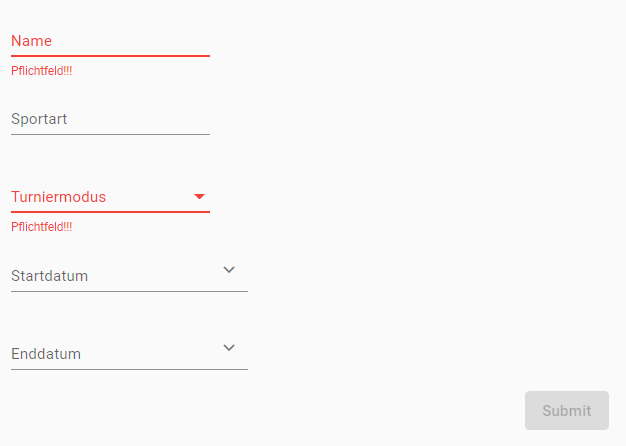
\includegraphics[scale=0.6]{pics/user-guide/tournament-create-page.PNG}
    \caption{Tournament-Details-Page}
\end{figure}

Diese Page ist zum Erstellen von Turnieren. Die Mindestanforderungen
sind hierbei nur ein Name und der Turniermodus.

Nachdem Sie ein Turnier erstellt haben erweitert sich die Tournament-Details-Page um die Funktion, Competitor(Spieler, Teams) für ein Turnier einzutragen.

\begin{figure}[H]
    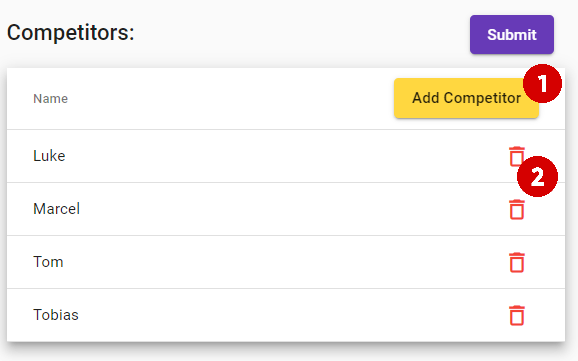
\includegraphics[scale=0.5]{pics/user-guide/tournament-add-player.PNG}
    \caption{Tournament-Details-Page mit Add-Player Funktion}
\end{figure}


\includegraphics[scale=0.05]{pics/user-guide/numbers/number-1.png} \begin{LARGE} Add Competitor \end{LARGE}

Bei Knopfdruck des Add-Competitor Button erscheint eine Liste aller Spieler die nicht in dem Team sind.
(\textit{Keine mehrfach Auswahl})

\begin{figure}[H]
    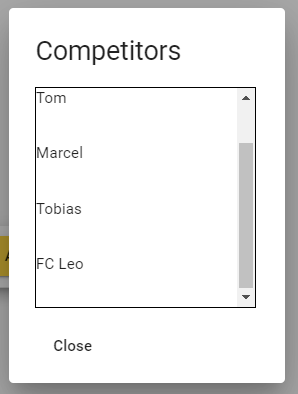
\includegraphics[scale=0.4]{pics/user-guide/add-competitor.PNG}
    \caption{Add-Player-PopUp (Tournament)}
\end{figure}


\includegraphics[scale=0.05]{pics/user-guide/numbers/number-2.png} \begin{LARGE} Actions \end{LARGE}

Mit dem Icon-Button 
\includegraphics[scale=0.3]{pics/user-guide/delete-icon.PNG} löschen Sie die Teilnahme eines Competitors für das Turnier. (\textit{Nicht den Competitor})

\newpage
\section{Match-Overview-Page - Rollen:Admin,Tournament-Organizer}
\begin{figure}[H]
    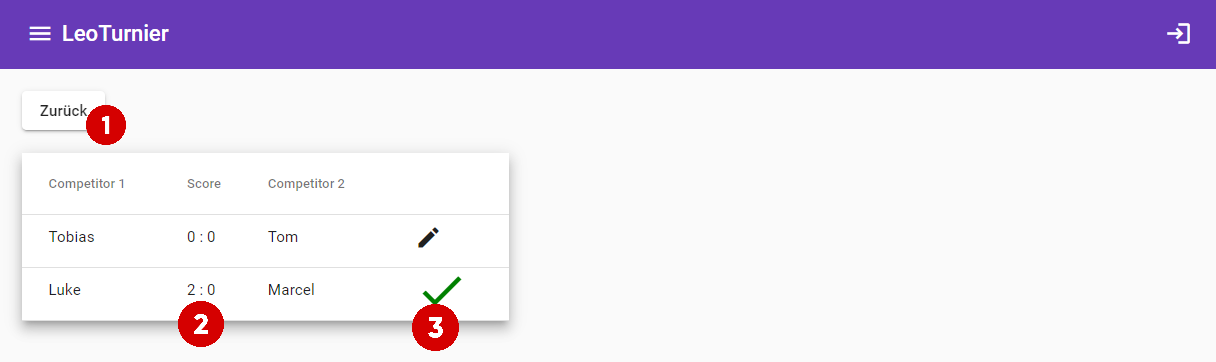
\includegraphics[scale=0.4]{pics/user-guide/match-overview-page.PNG} 
    \caption{Match-Overview-Page}
\end{figure}

\bigskip

\includegraphics[scale=0.05]{pics/user-guide/numbers/number-1.png} \begin{LARGE} Zurück-Button \end{LARGE}

Dieser Button leitet Sie zurück zur Tournament-Overview-Page.

\bigskip

\includegraphics[scale=0.05]{pics/user-guide/numbers/number-2.png} \begin{LARGE} Spiele \end{LARGE}

In dieser Tabelle werden alle Matches mit ihren beiden kontrahierenden Competitors und Spielstand angezeigt.  

\bigskip

\includegraphics[scale=0.05]{pics/user-guide/numbers/number-3.png} \begin{LARGE} Actions \end{LARGE}

Diese Spalte beinhaltet einen Icon-Button oder ein Icon:
\begin{itemize}
    \item \includegraphics[scale=0.3]{pics/user-guide/edit-icon.PNG}Updaten eines eines Matches (Sie werden danach zur Match-Submition-Page(5.7.1) geleitet)
    \item \includegraphics[scale=0.2]{pics/user-guide/finished-icon.PNG} Zeigt an dass, ein Spiel fertig gespielt ist .
\end{itemize}

\bigskip
\subsection{Match-Submition-Page}
\begin{figure}[H]
    \includegraphics[scale=0.6]{pics/user-guide/match-submition-page.PNG}
    \caption{Match-Submition-Page}
\end{figure}

\bigskip
\includegraphics[scale=0.05]{pics/user-guide/numbers/number-1.png} \begin{LARGE} Score-Tile \end{LARGE}

Die Match-Submition-Page enthaltet zwei Match-Tiles mit denen man den Score eines Spiels eintragen kann.
Der Punktestand kann entweder über eine Tastatureingabe, oder über die zwei Pfeile rechts neben dem Punktestand eingegeben werden.
Dabei muss der Spielstand eine Zahl zwischen 0-999 betragen.

(\textit{Mit einer so großen Spanne sollen mehr Sportarten möglich sein, da sich Punktestände von Sportart zu Sportart sehr stark ändern können z.B: Basketball (113-72) und Fußball(2-1)})

\bigskip
\includegraphics[scale=0.05]{pics/user-guide/numbers/number-2.png} \begin{LARGE} Submit-Score-Button \end{LARGE}

Bei Knopfdruck von Submit-Score wird der Punktestand geupdated und Sie werden zur Match-Overview-Page geleitet.

\bigskip
\includegraphics[scale=0.05]{pics/user-guide/numbers/number-3.png} \begin{LARGE} Finish-Match-Button \end{LARGE}

Bei Knopfdruck von Finish-Match wird der Punktestand geupdated und das Match beendet. Danach werden Sie zur Match-Overview-Page geleitet.

Da nun die Bedienung der App klar ist wird nun erklärt wie dabei das Frontend umgesetzt wurde.